\subsection{Thermal Simulations} \label{compvis_thermalsims}

    This section describes the thermal simulations undertaken to investigate the heat transfer phenomena associated with buried landmines.
    
    \subsubsection{Physical Principles}
    
        The thermal behaviour is governed by the unsteady heat equation. In three dimensions, the general form in Cartesian coordinates is:
        \begin{equation}
            c_p \rho \frac{\partial T}{\partial t} = 
            \frac{\partial}{\partial x} \left( k \frac{\partial T}{\partial x} \right) + 
            \frac{\partial}{\partial y} \left( k \frac{\partial T}{\partial y} \right) + 
            \frac{\partial}{\partial z} \left( k \frac{\partial T}{\partial z} \right)
        \end{equation}
        where:
        \begin{itemize}
            \item \( T(x,y,z,t) \) is the temperature field,
            \item \( k(x,y,z,t) \) is the thermal conductivity,
            \item \( \rho(x,y,z,t) \) is the mass density,
            \item \( c_p(x,y,z,t) \) is the specific heat capacity.
        \end{itemize}
        For piecewise constant properties, this can be written as
        \begin{equation}
            \frac{\partial T}{\partial t} = \alpha \left( \frac{\partial^2 T}{\partial x^2} + \frac{\partial^2 T}{\partial y^2} + \frac{\partial^2 T}{\partial z^2} \right)
        \end{equation}
        or, compactly,
        \begin{equation}
            \frac{\partial T}{\partial t} = \alpha \nabla^2 T,
        \end{equation}
        with the thermal diffusivity defined as \(\alpha := \frac{k}{\rho c_p}\).

    
    
    \subsubsection{Details of the Solver}
    
        The solver is a finite element solver implemented in MATLAB. The thermal model simulates heat conduction in a two-dimensional soil domain of dimensions $L =2$\,m $H = 1$\,m. The domain is defined as a rectangular region $\Omega_1$ representing the soil, with a circular inclusion $\Omega_2$ embedded within it to simulate the presence of a buried landmine. The mine is modelled as a circle with a radius of 0.05\,m and is located at coordinates (1.00\,m, 0.85\,m), which corresponds to a typical burial depth of 15\,cm. A structured finite element mesh is generated over the domain. For the high-resolution simulation a maximum mesh size of 0.005\,m is used (20 times smaller than the diameter of the mine), while a coarser mesh (maximum element size 0.02\,m) is employed during the iterative initial condition refinement. A mesh convergence study was conducted by lowering the maximum mesh size and observing no significant change in the peak temperature difference above the landmine.
        
        The transient heat conduction problem is solved using the Finite Element Method (FEM) with triangular linear Lagrange (P1) elements to discretise the spatial domain. The time-dependent heat equation is integrated using an implicit backward Euler scheme, which ensures numerical stability for large time steps. MATLAB's PDE Toolbox automatically assembles the mass and stiffness matrices and employs a sparse direct solver (UMFPACK) for the resulting system of equations. To optimise runtime, the simulation is split into two phases: a low-resolution 14-day phase to establish a steady state, followed by a high-resolution 24-hour phase for detailed thermal behaviour.
    
        \begin{figure}[htbp]
            \centering
            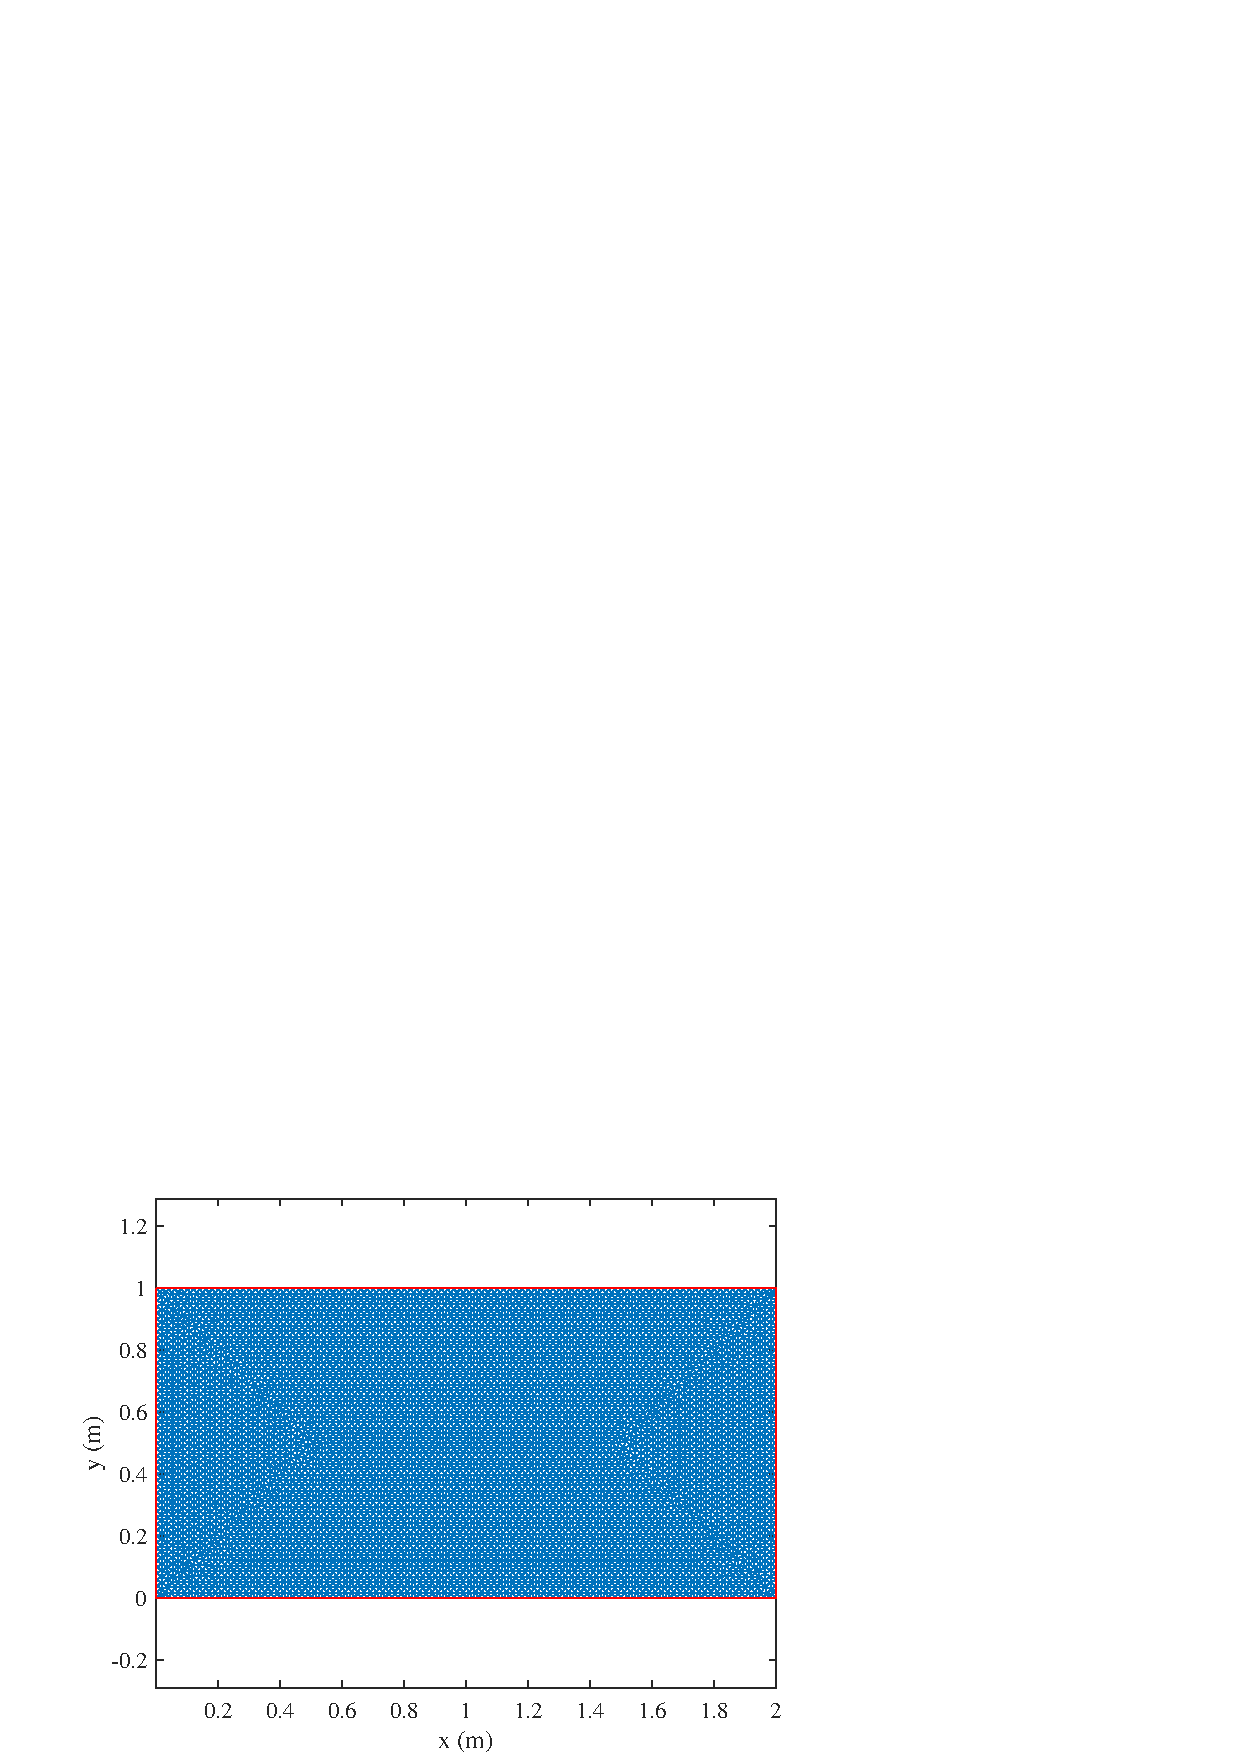
\includegraphics[width=0.8\textwidth]{figs/Rory/thermal_mesh.pdf}
            \caption{4x Downsampled thermal mesh - maximum mesh size 0.02m}
            \label{fig:thermal_mesh}
        \end{figure}
        
        
        
        \begin{figure}[htbp]
            \centering
            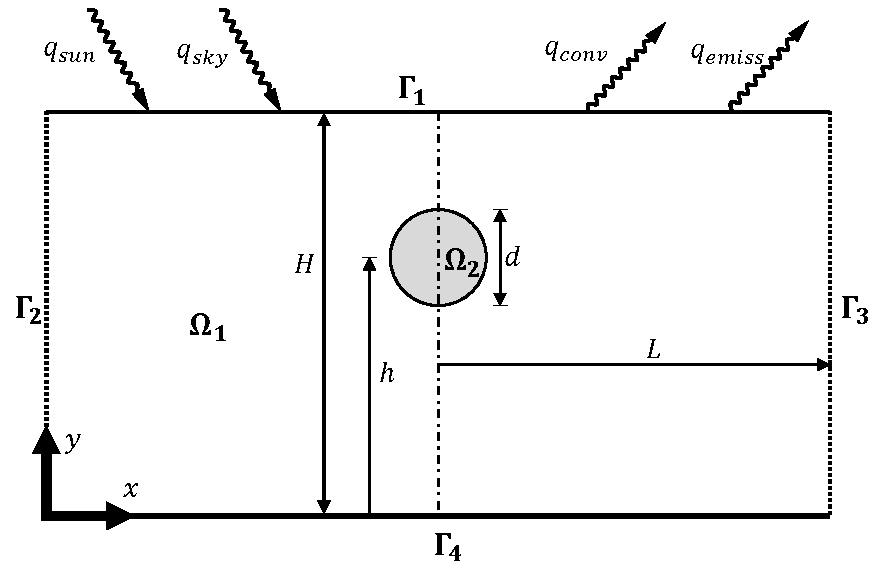
\includegraphics[width=0.8\textwidth]{figs/Rory/thermal_domain.pdf}
            \caption{Thermal simulation domain}
            \label{fig:thermal_domain}
        \end{figure}
    
    \subsubsection{Boundary Conditions} 
    
        The bottom boundary of the domain, $\Gamma_4$, is modelled as an isothermal Dirichlet condition, with the deep soil temperature $T_{\infty}$ set to the 30-day moving average air temperature, which approximates the thermal inertia of the soil. The left and right boundaries, $\Gamma_2$, $\Gamma_3$,  are modelled as adiabatic (zero heat flux) to prevent lateral heat exchange. This represents a symmetry condition, and implicitly assumes that lateral landmines are equally spaced. The top boundary, $\Gamma_1$,  is subject to a time-dependent Neumann boundary condition that accounts for:
    
        \begin{itemize}
        
            \item \textbf{Solar Insolation:} A periodic function models the diurnal variation of solar radiation for a given location and time of year. The solar flux is computed using explicit equations\footnote{\url{https://www.pveducation.org/pvcdrom/properties-of-sunlight/calculation-of-solar-insolation}} $\dot{q}_{sun}$
            
            \item \textbf{Convection:} Heat exchange with the ambient air is governed by convection, with the heat flux dependent on the wind speed and the temperature difference between the soil surface and the ambient air. Low-order correlations are used to model convection. I attempted to derive my own correlation using HLT, but was forced to use the correlations in HLT outside their domain, which produced dodgy results. Therefore, the recommended correlations from \cite{kahle1997model} were adopted, $\dot{q}_{conv} \approx \rho c_p C_D(w+2)(T - T_{\infty})$
            
            \item \textbf{Irradiance from the Sky:} Downward radiation from the sky is incorporated using an empirical relation, scaled by a water vapour pressure of 760\,mmHg \cite{nguyen2008inverse}. $\dot{q}_{\text{sky}} = T_{\infty} \left( 0.61 + 0.05 \sqrt{\omega} \right)^{0.25}$
            
            \item \textbf{Radiative Emission:} Longwave radiation loss is modelled using the Stefan-Boltzmann law, with an emissivity coefficient \(\epsilon = 0.9\) \cite{nguyen2008inverse}. $\dot{q}_{emiss} \approx \epsilon \sigma T^4$
            
        \end{itemize}
    
        The net heat flux leaving the soil is given by the location dependant Neumann boundary condition on the boundary $\Gamma_1$ : $\dot{q}_{net} = \epsilon \sigma T^4+ \rho c_p C_D(w+2)(T - T_{\infty}) - T_{\infty} \left( 0.61 + 0.05 \sqrt{\omega} \right)^{0.25}  - \dot{q}_{sun}$
    
    \subsubsection{Initial Conditions}

        The thermal field of the domain is initialised as homogeneous at the deep soil temperature (see Bottom Boundary). A lower resolution simulation (using a 0.02\,m mesh) is first run for a 24-hour period, after which the thermal field at the final time step is saved. This saved field is then used as the initial condition for a subsequent simulation. This process is iterated until the average temperature at the surface after 24hrs converges within a tolerance of 0.01\,\(^\circ\)C. The converged thermal field after 24 hours is subsequently used as the initial condition for the high-resolution simulation (0.005\,m mesh).

    \subsubsection{Simulation Setup for Afghanistan}
    
        For this study, the simulation is set up to replicate extreme environmental conditions found in Afghanistan. The solar insolation function is configured for a latitude of 33\(^\circ\) and conditions on 15th June, a month with almost no rainfall, ensuring reliable soil parameters. The wind speed is set at 4\,m/s. These conditions represent an extremum: extremely hot ambient soil temperatures combined with very dry, sandy soil (and hence low thermal diffusivity), such that the temperature rise is expected to be slight.
    
        \begin{table}[ht]
        \centering
        \caption{Mine, Soil and Ambient Properties (Dummy Values)}
        \label{tab:properties}
        \begin{tabular}{lccc}
        \hline
        \textbf{Parameter} & \textbf{Value} & \textbf{Units} & \textbf{Comments}\\
        \hline
        Mine Diameter d       & 0.1     & m    & Dummy value\\
        Mine Depth h          & 0.15   & m    & Typical burial depth\\
        Soil Thermal Conductivity $k_{\Omega_1}$ & 2  & W/(m$\cdot$K) & \cite{dummyRef1}\\
        Soil Density $\rho_{\Omega_1}$     & 1900     & kg/m$^3$ & \cite{dummyRef1}\\
        Soil Specific Heat Capacity $c_{p,{\Omega_1}}$  & 1480     & J/(kg$\cdot$K) & \cite{dummyRef1}\\
        Soil Thermal Diffusivity $\alpha_{\Omega_1}$ & $0.711$ & mm$^2$/s    & \cite{dummyRef2}\\
        Mine Thermal Conductivity $k_{\Omega_2}$ & 0.25  & W/(m$\cdot$K) & \cite{dummyRef1}\\
        Mine Density $\rho_{\Omega_2}$      & 1140     & kg/m$^3$ & \cite{dummyRef1}\\
        Mine Specific Heat Capacity $c_{p,{\Omega_2}}$ & 1980     & J/(kg$\cdot$K) & \cite{dummyRef1}\\
        Mine Thermal Diffusivity $\alpha_{\Omega_2}$ & 0.111 & mm$^2$/s    & \cite{dummyRef2}\\
        Maximum Surface Temperature & XX & K    & Dummy value\\
        Minimum Surface Temperature & XX & K    & Dummy value\\
        Wind Speed          & 4      & m/s  & \cite{dummyRef2}\\
        \hline
        \end{tabular}
        \end{table}
    
        Justification for using the properties of TNT to represent the entire landmine is based on the fact that most landmines contain little to no metal—apart from the firing pin—and are primarily composed of high explosives very similar in composition to TNT. Afghanistan was chosen as the simulation environment because it represents an extreme environmental condition that is ideal for validating our computer vision (CV) model, and because the region is known to have a high density of mines (XX in the world).

    \subsubsection{Results and Validation}
    
        Preliminary results indicate a peak temperature difference (delta-\(T\)) and an optimum time of day at which the thermal contrast is maximised. These results are compared with those reported in other studies (e.g., \cite{dummyRef3}) to validate the simulation. The findings suggest that the chosen thermal sensor (see HUIRUI section) is capable of detecting buried landmines even under extreme environmental conditions. When combined with the CV analysis and the detectability hypothesis, the results provide strong evidence for the effectiveness of the sensor in field applications.
    
        \begin{figure}[htbp]
            \centering
            \begin{minipage}[b]{0.48\textwidth} % Adjust width as needed
                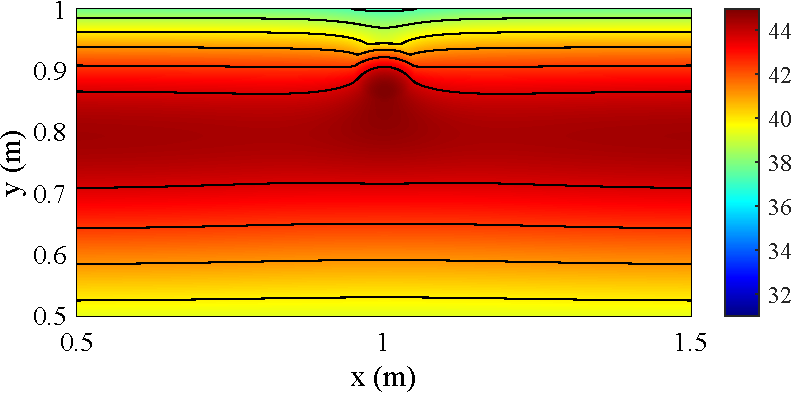
\includegraphics[width=\textwidth]{figs/Rory/thermal_result.pdf}
                %\caption{Enlarged simulation domain at local Afghanistan time midnight} % Remove individual caption
                %\label{fig:thermal_result} % Remove individual label
            \end{minipage}
            \hfill % Add horizontal space between the figures
            \begin{minipage}[b]{0.48\textwidth} % Adjust width as needed
                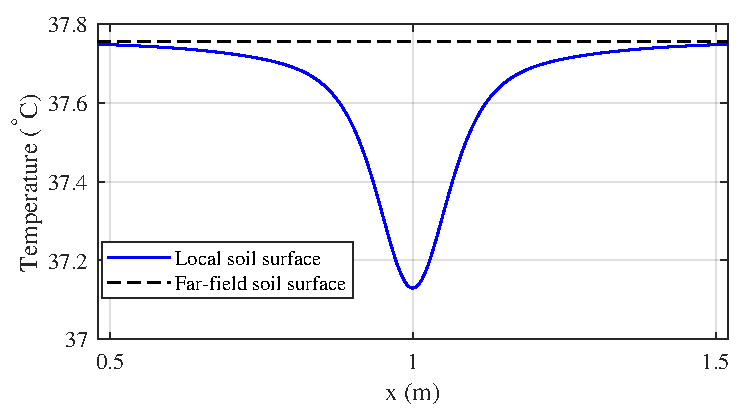
\includegraphics[width=\textwidth]{figs/Rory/1D_distribution_cropped.pdf}
                %\caption{Surface distribution} % Remove individual caption
                %\label{fig:thermal_1D} % Remove individual label
            \end{minipage}
            \caption{Converged initial condition plotted both as a 2D contour plot of a zoomed section of the domain (left), and a 1D line plot of the surface distribution over the same x-axis (right).}
            \label{fig:combined_thermal} % Add a combined label
        \end{figure}
    
    
    \subsubsection{Sensitivity Analysis}
    
        A sensitivity analysis was carried out to assess the impact of variations in key parameters, such as soil conductivity, ambient temperature, mine depth, and mine diameter. The analysis further involves generating fuzzy rules for an Adaptive Neuro-Fuzzy Inference System (ANFIS) to better understand the influence of these parameters on the detectability of buried landmines.
        
        \begin{figure}[htbp]
            \centering
            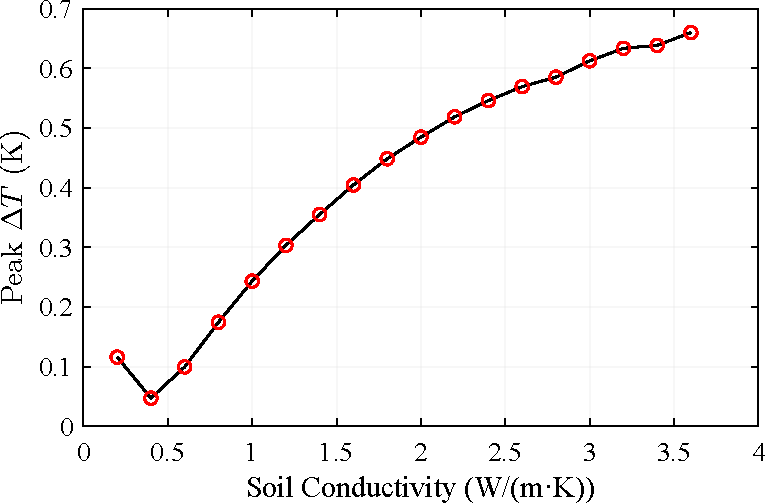
\includegraphics[width=0.8\textwidth]{figs/Rory/thermal_sensitivity_conductivity.pdf}
            \caption{Effect of varying soil conductivity on the peak $\Delta T$ value over one day}
            \label{fig:thermal_sensitivity_conductivity}
        \end{figure}
    
    